\documentclass[11pt]{amsart}
\usepackage{geometry}
\geometry{a4paper, left=1.5cm, right=1.5cm, top=1.5cm, bottom=1.5cm}
\usepackage{graphicx}
\usepackage[export]{adjustbox}
%\usepackage{tikz}
\usepackage{amssymb}
%\usepackage{epstopdf}
\usepackage{minted}
\usepackage[dvipsnames]{xcolor}
\usepackage{hyperref}
%\DeclareGraphicsRule{.tif}{png}{.png}{`convert #1 `dirname #1`/`basename #1 .tif`.png}
\hypersetup{
    colorlinks=true,
    linkcolor=blue,
    filecolor=magenta,
    urlcolor=cyan,
}
\usepackage{comment}
\title[OpenMP]{OpenMP Assignment}
\author[]{Dr. Pascal Elahi (PawseySC)}
%\date{}                                           % Activate to display a given date or no date

\begin{document}
\maketitle
\pagestyle{plain}
The assignment is to use a simple \textbf{N-Body} gravitational code. 

Here we provide:
\begin{enumerate}
	\item[\S\ref{sec:nbody}:] An overview of the N-Body code. If familiar with N-Body codes, please continue to \S\ref{sec:code}.
	\item[\S\ref{sec:code}:] An overview of the code repository. 
  \item[\S\ref{sec:tasks}:] The assessable tasks.  
\end{enumerate}


\section{N-Body}
\label{sec:nbody}
In physics and astronomy, an N-body simulation is a simulation of a dynamical system of particles, usually under the influence of physical forces, such as gravity. N-body simulations are widely used tools in astrophysics for investigating the dynamics of few-body systems like the solar system to understanding the evolution of the large-scale structure of the universe. They are also used to module fluids using smooth-particle hydrodynamics. 

\par 
This approach for discretisation is often referred to as a Lagrangian approach, where the observer follows an individual fluid parcel as it moves through space and time. The evolution of an individual particle's position gives the pathline of the parcel. 

\par 
This in contrast to Eulerian specifications of the flow field. Here fluid motion is evaluated at specific locations in the space, often evaluated using a mesh. This mesh can be regular or irregular, fixed or adaptive. 

\par 
An common use-case for an N-Body simulation is to follow the non-linear evolution of structure formation such as galaxy filaments and galaxy halos from the influence of dark matter on cosmological scales. An example of the output from the N-Body code provided in this assignment that mimics the distribution of matter in cosmological simulation is provided in Fig.~\ref{fig:nbody-distribution}.
\begin{figure}[!h]	
	\centering
	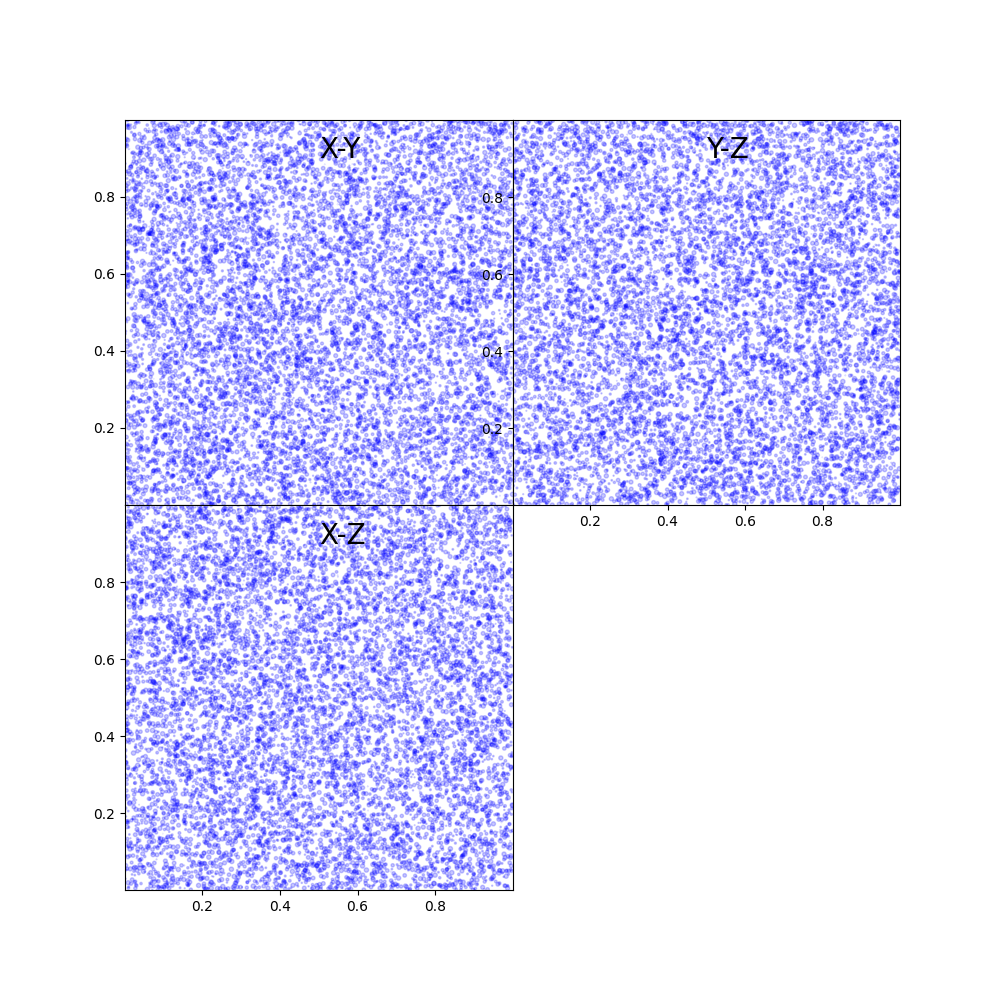
\includegraphics[width=0.4\textwidth, valign=c, clip=true, trim=2.cm 2.cm 2.cm 2.cm]{figs/nbody-scatter-plot.t-0.png}
	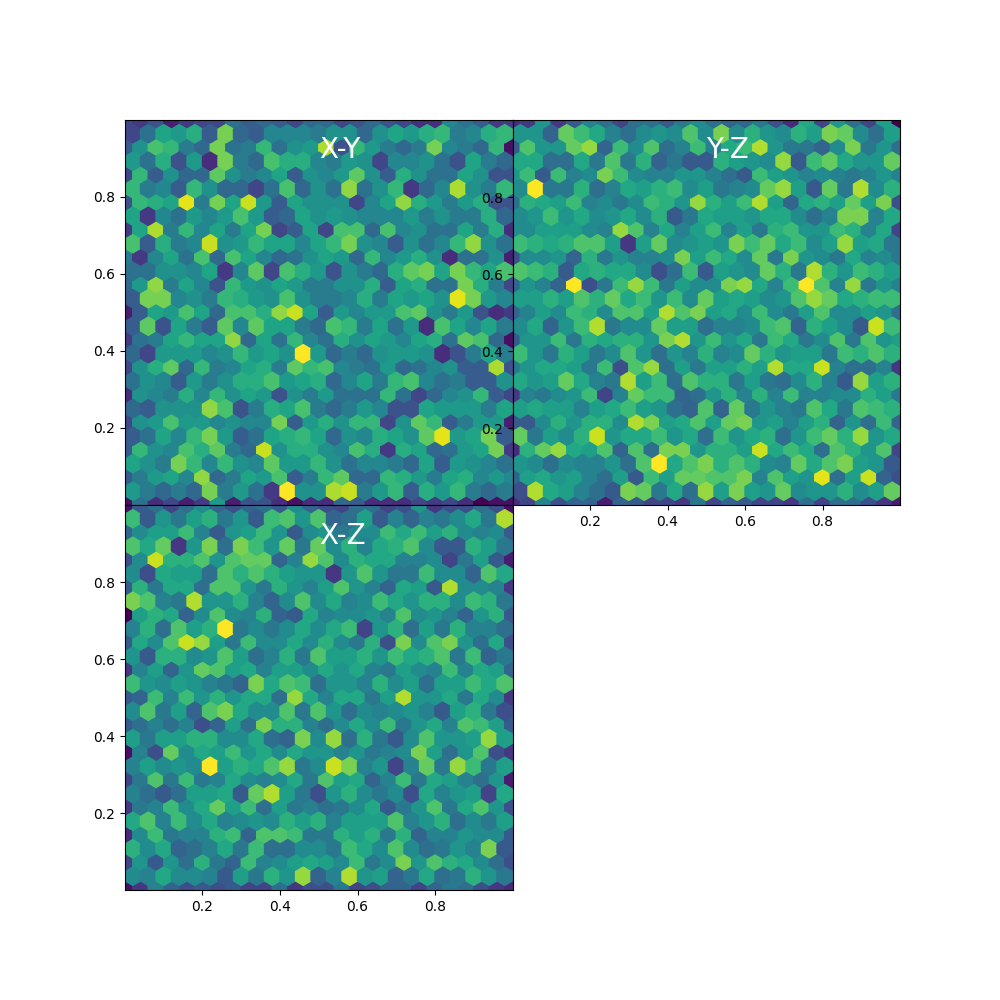
\includegraphics[width=0.4\textwidth, valign=c, clip=true, trim=2.cm 2.cm 2.cm 2.cm]{figs/nbody-density-plot.t-0.png}
	\caption{An example of a random particle distribution and the corresponding projected density field. We show $X-Y$, $X-Z$ and $Y-Z$ projections.}
	\label{fig:nbody-distribution}
\end{figure}

\par 
The basics of the computation for evolving particles at each individual time-step $\Delta t$ of the simulation are as follows:
\begin{itemize}
	\item {\color{ForestGreen}Acceleration} Calculate the acceleration, $\vec{a}_{\textrm{new}}$, on each individual particle. A simple N-body code can involve calculations that scale as $N^2$, where $N$ is the number of particles.
	\item {\color{CornflowerBlue}Velocity Update} Update the momentum of all the particles based on these forces, \\$\vec{p}_{\textrm{new}} = \vec{p}_{\textrm{old}} + \vec{a}_{\textrm{new}}\Delta t$
	\item {\color{Purple}Position Update} Update the positions of all the particles based on these momenta, \\$\vec{x}_{\textrm{new}} = \vec{x}_{\textrm{old}} + \vec{p}_{\textrm{new}}\Delta t$
\end{itemize}
There are issues with this simplified approach related to energy conservation primarily related to the time step. One can also use other techniques to reduce errors in the time-integration. 

\subsection{Impact of Time-steps}
\label{sec:nbody:timestep}
The time-integration technique is critical to conserving the total energy of the system and having the correct evolution. For example, the N-Body code provided in this assignment can evolve a system with a fixed time step or an adaptive time step. A poorly chosen fixed time step can result in the simulation not correctly evolving the system when the dynamical time is short, such as in close encounters of particles evolving under gravity as seen in Fig.~\ref{fig:nbody-orbits}. 
\begin{figure}[!h]	
	\centering
	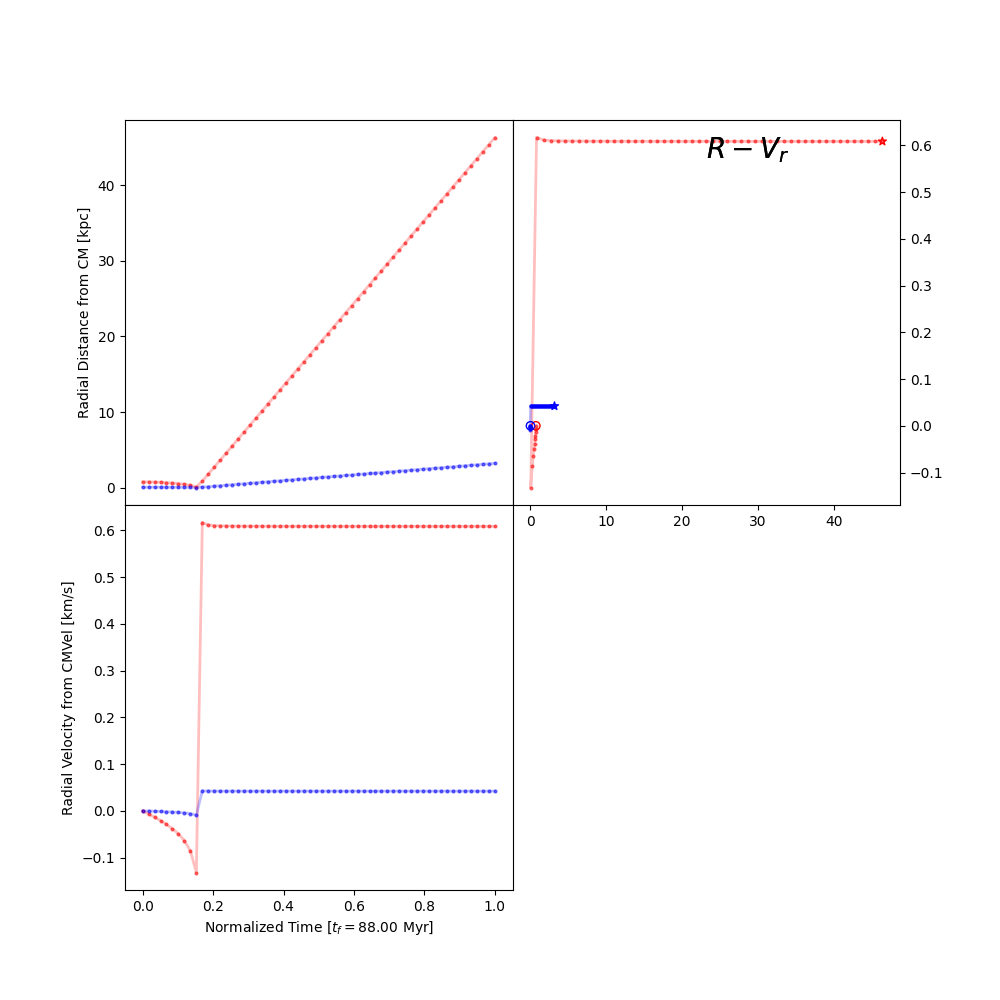
\includegraphics[width=0.4\textwidth, valign=c, clip=true, trim=2.cm 2.cm 2.cm 2.cm]{figs/nbody-phase-plot-rad-static.png}
	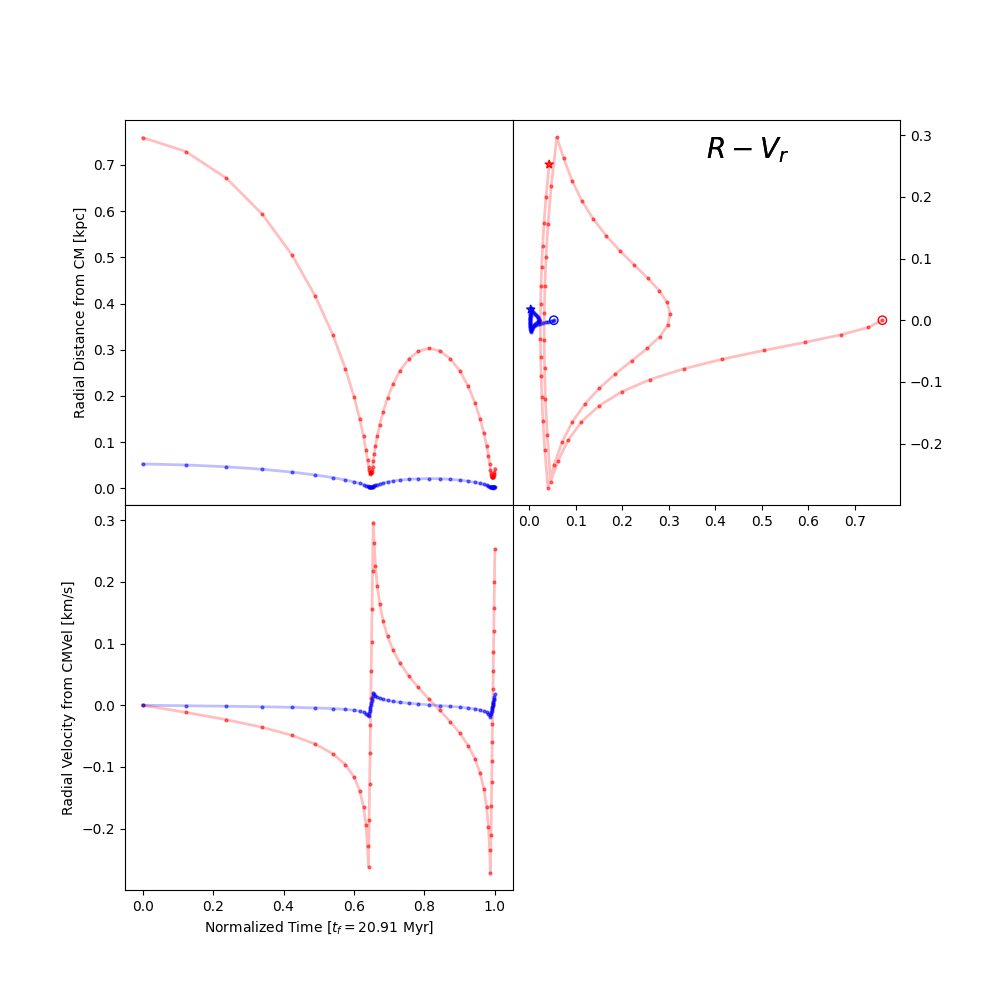
\includegraphics[width=0.4\textwidth, valign=c, clip=true, trim=2.cm 2.cm 2.cm 2.cm]{figs/nbody-phase-plot-rad-adaptive.png}
	\caption{Phase-space plots: We show an example of the impact time-steps can have on the evolution of the system comparing fixed time steps (left) to adaptive time steps (right).}
	\label{fig:nbody-orbits}
\end{figure}

\par 
Here we follow the radial position and velocity of two particles, one more massive (blue) than the other (red). The system is initialized such that the particles are in orbit around the common centre-of-mass. For the fixed time step, the simulation does not correctly follow the close encounter, moving the particle too much during this phase, resulting the lighter particle's having too much momentum after the encounter and streaming off unbound from the system as see in the left panel. 

\par 
An adaptive time step which is always set to some small fraction of the dynamical time of the system will correctly model the encounter. However, it is worth noting here that there are still issues with the energy of the system (see assignment questions). 

\subsection{Long-range forces}
\label{sec:nbody:longrange}
There are several challenges to modelling long-range forces. Long-range forces like the gravitational force are computationally expensive as the calculations scale as $\mathcal{O}(N^2)$, that is one must calculate the force between each pair of particles. Computational techniques can be used to reduce the scaling but require some approximations to be made (see assignment questions).

\par 
Correctly solving the force for periodic systems requires additional corrections as it is not computationally feasible to simple add more pairs where one has been shifted by the period. Such an approach would require terminating the number of additional particles out to some multiples of the period, introducing additional approximations. Instead, a typical approach is to break the force calculation into a shorter range and long (period) range set, often referred to as Ewald summation (\href{see https://en.wikipedia.org/wiki/Ewald_summation}). 

\par 
Finally, there is added complexity to correctly calculating the true evolution of the system given the finite-speed of the force carrier. To accurately calculate long-distance forces a full general relativistic approach is required \cite{grnbody}. However, the difference between the accurate solution and an approximateive one where the force is transitted instantaneously can be small for forces that depend on radial distance of the form $r^{n}$, $n\leq-2$ since the long-range forces are small\cite{grcorrections}.

\subsection{Short-range forces}
\label{sec:nbody:shortrange}
Short range forces also face several challenges. The first is that the naive implementation would require 
$\mathcal{O}(N^2)$ radius calculation to see if a pair is within the short-range force before calculating said force. Computational techniques can be used to significantly reduce the computational cost of the local neighbour search, without requiring any approximations (see assignemnt questions).

\par 
These forces can also be subject to the speed of the force carrier and may also require corrections to accurately calculate the force. 

\section{Code Repository}\label{sec:code}
The code that forms the basis of the assignment contains the following 
\begin{itemize}
	\item basic files like a README, License
	\item \texttt{Makefile} setup to compile codes with a variety of different flags and features. For a quick tutorial on GNU Make, see \href{https://www.gnu.org/software/make/}{here}. Students are expected to be familiar with Make and the associated commands. Please familiarise yourself with this material. 
	\item source code in \texttt{src/*f90} (\texttt{Fortran}). 
	\item bocumentation and \LaTeX\ source code in \texttt{docs}
	\item python scripts for visualisation. 
\end{itemize}
To familiarise yourself with the contents you can see what make options are available and browse the source directory. 
\begin{center}
\begin{minipage}{0.95\textwidth}
\small
\begin{minted}[frame=single,]{sh}
make allinfo # provides all the information of the commands listed below  
make configinfo # provides the different options available 
make makecommands # what you can make by typing these commands
make buildinfo # current compilers used
\end{minted}
\end{minipage}
\end{center}
You'll note that the make file is setup to accept command line arguments that can set compiler families such as \texttt{GCC}, \texttt{CRAY-GNU}, \texttt{CRAY} when you type \texttt{make configinfo}. Try the following
\begin{center}
\begin{minipage}{0.95\textwidth}
\small
\begin{minted}[frame=single,]{sh}
# use the GNU CC family of compilers, gcc, g++, & gfortran AND 
# compile the serial version of the code, both C and Fortran sources.
make COMPILERTYPE=GCC cpu_serial 
# use the GNU family of compilers with the Cray compiler wrappers 
# on Setonix and compile the openmp source codes (if present)
make COMPILERTYPE=CRAY-GNU cpu_openmp 
\end{minted}
\end{minipage}
\end{center}


\subsection{Source}
The common function calls with interfaces are listed in \texttt{src/common.f90} provides a module with the same set of interfaces and subroutines. 
\begin{center}
\begin{minipage}{0.95\textwidth}
\small
\begin{minted}[frame=single,]{fortran}
module nbody_common
    type Particle
        integer(8) :: ID
        real(8) :: mass
        real(8) :: radius
        real(8) :: position(3)
        real(8) :: velocity(3)
        real(8) :: accel(3)
        integer(8) :: PID
    end type Particle

    !   ascii mesh visualisation
    subroutine visualise_ascii_mesh(opt, step, parts)
    !   ascii visualisation (not implemented in full)
    subroutine visualise_ascii(opt, step, parts)
    ! no visualisation
    subroutine visualise_none(step)
    ! visualisation routine
    subroutine visualise(opt, step, parts)
    ! generate random IC
    subroutine generate_rand_IC(opt)
    ! generate random orbiting particles IC
    subroutine generate_orbit_IC(opt)
    ! generate IC
    subroutine generate_IC(opt, parts)
    ! UI
    subroutine getinput(opt)
    ! get some basic timing info
    real*8 function init_time()
    ! get the elapsed time relative to start
    subroutine get_elapsed_time(start)
end module
\end{minted}
\end{minipage}
\end{center}

\newpage
The main program consists of : 
\begin{center}
\begin{minipage}{0.95\textwidth}
\begin{minted}[frame=single,]{fortran}
    ! generate particles 
    call generate_IC(opt, parts)
    time1 = init_time()
    current_step = 0
    print *, "Running simulation for ", opt%nsteps
    ! run time integration for certain number of steps
    do while (current_step .ne. opt%nsteps)
            time2 = init_time()
            ! visualise if necessary 
            call visualise(opt, current_step, parts)
            ! produce output if necessary 
            call nbody_output(opt, current_step, parts)
            ! calculate acceleration 
            call accel_update(opt, parts)
            ! calculate velocity 
            call velocity_update(opt, parts)
            ! calculate positions 
            call position_update(opt, parts)
            ! update time 
            opt%time = opt%time + opt%time_step
            current_step = current_step + 1
            call get_elapsed_time(time2)
            time2 = init_time()
    end do 
    write(*,*) "Finished NBody simulation"
    call get_elapsed_time(time1);
\end{minted}
\end{minipage}
\end{center}
Implementations of the 3 main integration functions are present in the code. Familiarise yourself with these functions. 

\par 
Running the code is relatively simple  
\begin{center}
\begin{minipage}{0.95\textwidth}
\small
\begin{minted}[frame=single,]{sh}
make cpu_serial
./bin/01_cpu_serial 
Usage: <number of particles> <nsteps>
 [<Boundary type> <IC type> <Time Step Criterion> <Visualisation type> <Vis res>]
# simulation of 1e3 particles in periodic box with adaptive time step for 100 steps  
./bin/01_cpu_serial 1000 100 1 0 1  
\end{minted}
	% 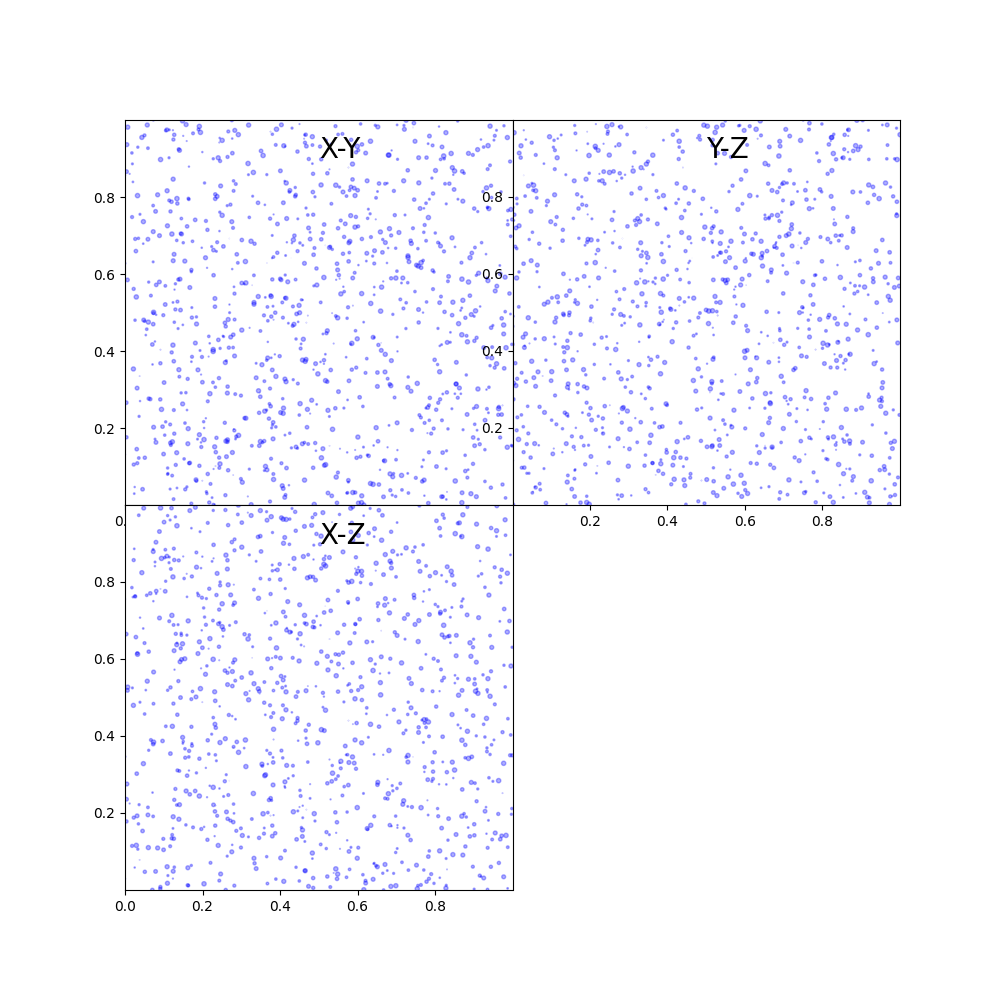
\includegraphics[width=0.4\textwidth, valign=c, clip=true trim=40.cm 2.cm 20.cm 2.cm]{figs/nbody-scatter-plot.t-i.png}
	% 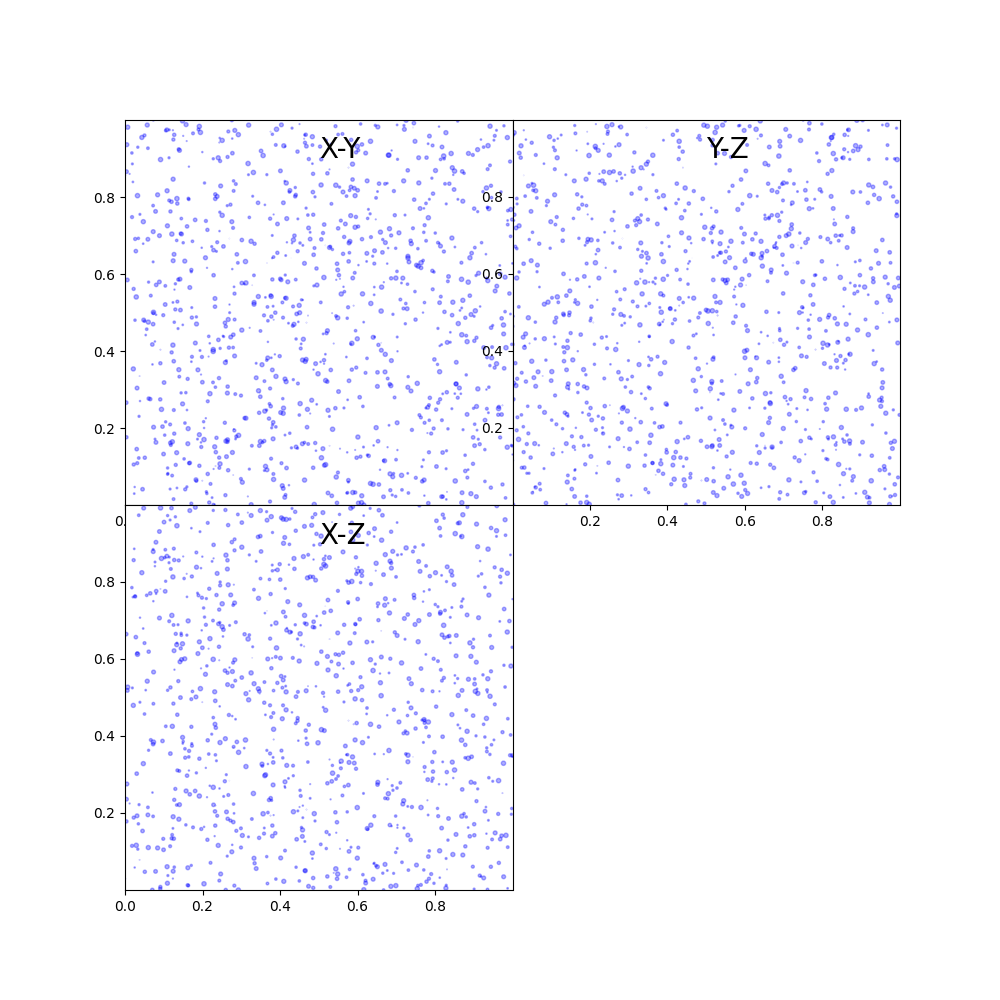
\includegraphics[width=0.4\textwidth, valign=c, clip=true trim=2.cm 2.cm 2.cm 2.cm]{figs/nbody-scatter-plot.t-f.png}
	% 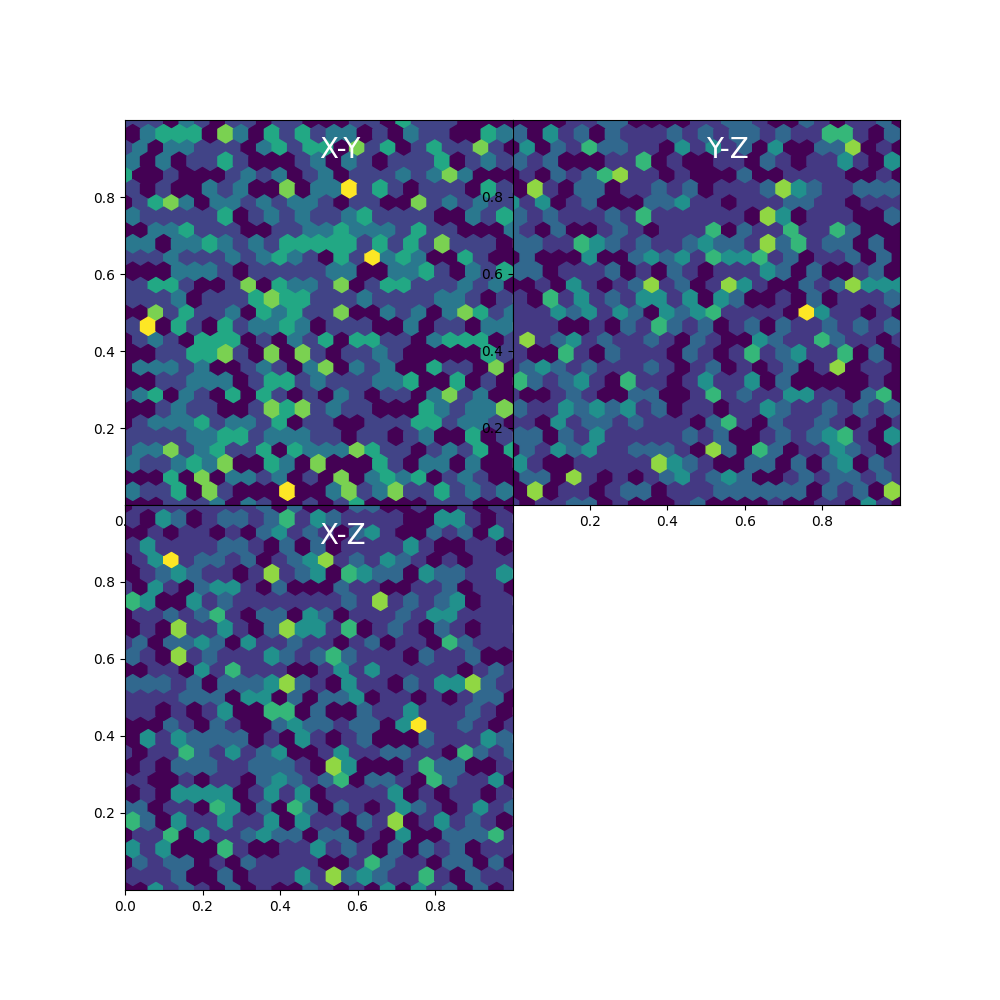
\includegraphics[width=0.4\textwidth, valign=c, clip=true trim=2.cm 2.cm 2.cm 2.cm]{figs/nbody-density-plot.t-i.png}
	% 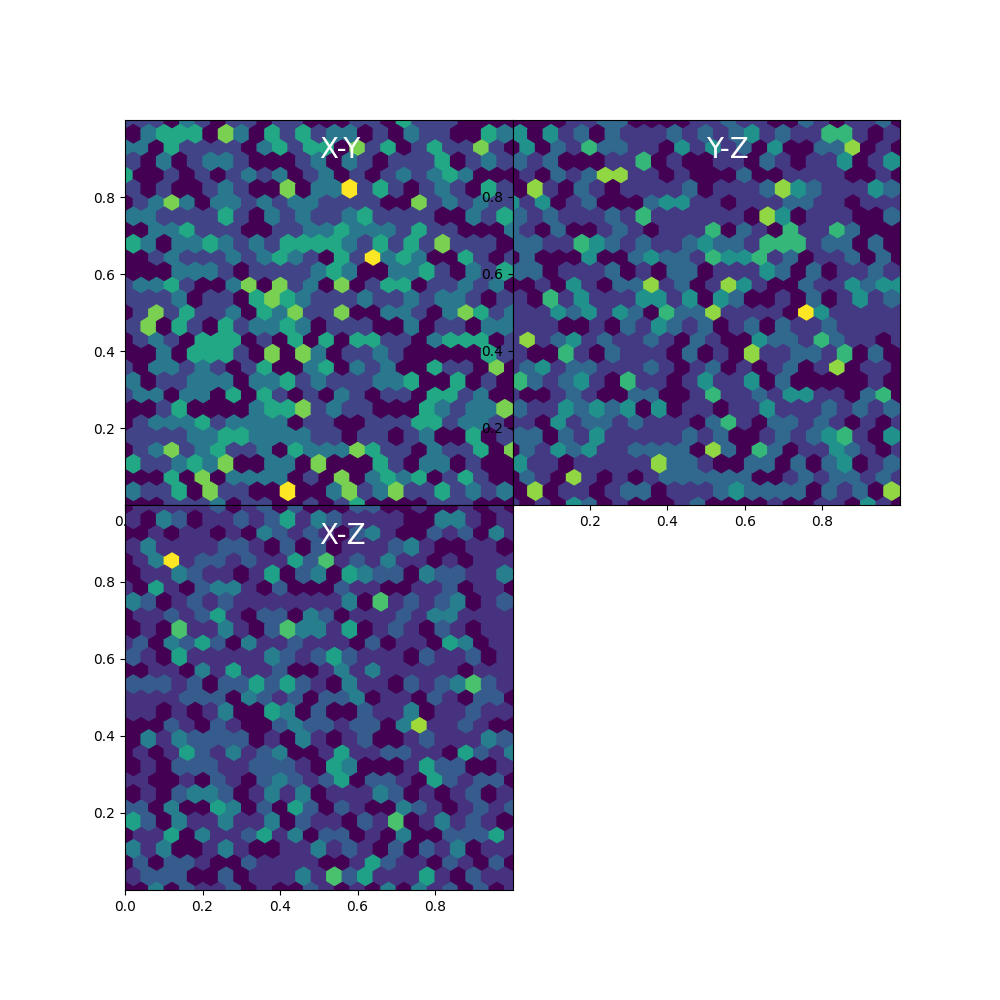
\includegraphics[width=0.4\textwidth, valign=c, clip=true trim=2.cm 2.cm 2.cm 2.cm]{figs/nbody-density-plot.t-f.png}
\end{minipage}
\end{center}

\subsection{Compiling on Pawsey systems}
The serial fortran codes will compile with all compilers on \texttt{setonix} so long as the appropriate compiler for the given programming environment is chosen. The make commands to use are 
\begin{itemize}
    \setlength{\itemindent}{70pt}
    \item[\texttt{PrgEnv-cray}:\quad]{\texttt{make COMPILERTYPE=CRAY}}
    \item[\texttt{PrgEnv-gnu}:\quad]{\texttt{make COMPILERTYPE=CRAY-GNU}}
\end{itemize}
On other machines that do not make use of the Cray compiler wrappers, it is just a matter of specifying the appropriate compiler such as \texttt{make COMPILERTYPE=GNU} for \texttt{gnu} compilers.


\newpage
\section{Assessable Tasks}\label{sec:tasks}
\begin{center}
  \large
  The assignment will consist of providing a report testing and profiling the OpenMP-enabled N-Body code and provide the updated source code. 
  \textbf{The PDF report and the archive of the full source code should be sent to (or shared via a url) to my email \href{mailto:pascal.elahi@pawsey.org.au}{pascal.elahi@pawsey.org.au}. }
\end{center}
\subsection*{How to start?\nopunct\\} \label{sec:tasks:staring}
For each task, start by profiling the code using \texttt{gprof}. This will allow you to identify where most of the time is spent. Try using large grid sizes (within reason). With this profiling information, you should be able to identify what should be parallelised. Look at the code itself and make sure you understand the algorithm.

Copy the original serial source file to \texttt{02\_nbody\_cpu\_openmp\_loop} and/or \texttt{02\_nbody\_cpu\_openmp\_task} and try compiling the code
\begin{center}
\begin{minipage}{0.95\textwidth}
\begin{minted}[frame=single,]{sh}
cp src/01_nbody_cpu_serial.f90 src/02_nbody_cpu_openmp_loop.f90
cp src/01_nbody_cpu_serial.f90 src/02_nbody_cpu_openmp_task.f90
\end{minted}
\end{minipage}
\end{center}
Profile the code using tools like gprof or just using the timing routines in-built in the code. 
Here the example is for building on setonix.
\begin{center}
\begin{minipage}{0.95\textwidth}
\begin{minted}[frame=single,]{sh}
# compile
make COMPILERTYPE=CRAY-GNU PROFILER=ON cpu_openmp_loop
# run two steps of a moderately large number of particles 
./bin/02_nbody_cpu_openmp_loop 100000 2
# profile
gprof -lbp ./bin/02_nbody_cpu_openmp_loop gmon.out > analysis.txt
\end{minted}
\end{minipage}
\end{center}
Look at the output produced by the code as well as the output of the profiling. The code provides the state of every particle at every step, saved as {\color{blue}\texttt{nbody-data.txt}}. The code also writes to standard out, so when running save the output to meaningful log files. Similarly save the output file to a meaning filename.
\begin{center}
\begin{minipage}{0.95\textwidth}
\begin{minted}[frame=single,]{sh}
# lets set some variables for a run. Here numbers are examples only.
nomp=2
np=1000
nsteps=10
# set some meaningful name. Could be reference, latests, etc.
someversionname=reference
# set a base name
basename=nbody-${someversionname}.nomp-${nomp}.np-${np}.nsteps-${nsteps}
export OMP_NUM_THREADS=${nomp}
./bin/02_nbody_cpu_openmp_loop ${np} ${nsteps} > ${basename}.log
mv nbody-data.txt ${basename}.data.txt
\end{minted}
\end{minipage}
\end{center}
In this way, you can compare results as you update the code, change the number of threads, change versions, etc and keep track of changes in performance and compare results.

\subsection{{\color{Red} Preliminaries}: Serial optimisation\nopunct\\}\label{sec:tasks:serialopt}
The code is not optimised serially. Please look at the code, particularly the main subroutines to improve the performance and show that this is the case. 

\subsection{{\color{Red} Principle Task}: Implement OpenMP Parallelism\nopunct\\}\label{sec:tasks:omp}
Perform an OpenMP parallelisation of the serial code, test performance and scaling. There are two main approaches, {\color{Orange}\textbf{Loop}} and {\color{Orange}\textbf{Task}} parallelism. This source code should be called \texttt{02\_cpu\_openmp\_loop.f90} or for task parallelism  \texttt{02\_cpu\_openmp\_task.f90}. One can 

The code should contain extensive \textbf{\textit{comments}}, noting what you are doing \textit{and why}. I will compile your code using the appropriate \texttt{make} command.
{\centering \textit{You must show that the code produces correct results regardless of the number of OpenMP threads used. This can be checked with the output file.}}

\subsection{{\color{Red}Secondary Task}: Scaling Tests\nopunct\\}\label{sec:tasks:scaling}
Test how the code scales with number of threads and also problem size and discuss the observed behaviour. Start with a few particles and incraese it. Increase the number of OpenMP threads from 1 to 16 (taking note of the number of actual logical cores on the system). Note that visualising each step significantly impacts the speed of the program, so we suggest running with visualisation turned off (this is the default) and even commenting out the \texttt{nbody\_output} subroutine.

\par 
Compare your results and explain the scaling seen both with problem size and number of threads. Please keep in mind that when running the scaling tests, submit sbatch jobs requesting access on the work queue of Setonix for a short amount of time.

\subsection{{\color{Red}Third Task}: Discussion Questions\nopunct\\}\label{sec:tasks:discussion}
Answer the following 3 questions in the assignment.
\begin{enumerate} 
  \item Discuss how the algorithm for calculating the gravitational force can be improved in regards to how the computational cost. How would that impact the code and the resulting simulation?
  \item Discuss how the algorithm for calculating the short range collisional force can be improved in regards to how the computational cost. How would that impact the code and the resulting simulation?
  \item Discuss how the time-integration could be improved to improve the accuracy of the simulation without drastically decreasing the time-step and increasing the number of steps taken. How would that impact the code and the resulting simulation? 
\end{enumerate}

\section{{\color{Blue}What you need to hand in\nopunct\\}}\label{sec:handin}

You must submit a zip (or tar) file containing:
\begin{itemize}
  \item Your code within the repository so that it can be easily compiled. Make it clear which type of OpenMP parallelisation you have implemented.
  \item A pdf of your code so that I can read it and the comments associated with the changes you have made. Remember to be verbose!
  \item A pdf report discussing the OpenMP parallelisation of the code and answer the discussion questions above. Details of what should be in the report are outlined below.
\end{itemize}

\subsection*{Report\nopunct\\}\label{sec:handin:report}
\noindent Your report should contain the following sections:
  \begin{enumerate}
  \item{\textbf{Intro} : Describe compilers used, any additional compilation flags used such as optimisation. Describe choice of parallelism used (if applicable).} 
  \item{\textbf{Profiling} : Profile the code and discuss the results.}
  \item{\textbf{Correctness} : Show code compiles and still produces correct results compared to serial version. Ensure that all functionality of the code remains intact. If you wish, you can add functionality.}
  \item{\textbf{Implementation} : Describe and discuss serial optimisation, openmp implementation, all choices and any testing that has driven a choice.}
  \item{\textbf{Scalability} : Test how the code performs, show scaling of code and discuss results.}
  \item{\textbf{Code} : Highlight changes to code.}
  \item{\textbf{Discussion Questions} : Answer the 3 questions posed above}
\end{enumerate}

\subsection*{Marks\nopunct\\}\label{sec:handin:marks}
\noindent The assignment is marked out of \textbf{36}. The marks are awarded as follows:
\begin{itemize}
  \item{\textbf{Correctness} : The code must compile and produce the correct result. \textbf{Otherwise a factor of 1/2 will be applied to the code related sections, which total 30 marks.}}
  \item{\textbf{Profiling} : Out of 2}
  \item{\textbf{Implementation} and \textbf{Code}: Out of 20}
  \item{\textbf{Scalability}: Out of 8}
  \item{\textbf{Discussion Questions}: Out of 6}
\end{itemize}

\noindent{\color{CornflowerBlue}BONUS}: \textit{If Both Task and Loop are implemented, bonus marks will be awarded.}

  %\item {\color{CornflowerBlue}BONUS}: Discuss how does thread affinity affects performance.
  %\item {\color{CornflowerBlue}BONUS}: Show that the code is also vectorised and how this affects performance.

\bibliographystyle{plain}
\begin{thebibliography}{2}

\bibitem{enzo} Bryan, G.~L., Norman, M.~L., O'Shea, B.~W., et al.\ 2014, \textit{Astrophysical Journal Supplementary Series}, 211, 19. doi:10.1088/0067-0049/211/2/19

\bibitem[Adamek et al.(2013)]{grnbody} Adamek, J., Daverio, D., Durrer, R., et al.\ 2013, \textit{Physical Review Letters}, 88, 103527. doi:10.1103/PhysRevD.88.103527

\bibitem[East et al.(2018)]{grcorrections} East, W.~E., Wojtak, R., \& Abel, T.\ 2018, \textit{Physical Review Letters}, 97, 043509. doi:10.1103/PhysRevD.97.043509

\end{thebibliography}

\end{document}
